\chapter{Stokes Matrizen}
\begin{comment}
Matrizen Sicht:
\begin{itemize}
  \item \cite[Chapter 3]{boalch}
    \\ largely following:
    \begin{itemize}
      \item[\textbf{8}] D.G. Babbitt and V.S. Varadarajan.
      \textbf{Formal reduction theory of meromorphic differential equations: a
        group theoretic view.}
      \texttt{euclid.pjm.1102720203.pdf}
      \item[\textbf{11}] W. Balser, W.B. Jurkat, and D.A. Lutz.
      \textbf{Birkhoff invariants and Stokes’ multipliers for meromorphic
        linear differential equations.}
      \item[\textbf{40}] M. Jimbo, T. Miwa, and Kimio Ueno.
      \textbf{Monodromy preserving deformations of linear differential
        equations with rational coefficients I.}
      \item[\textbf{43}] M. Loday-Richaud
      \textbf{Stokes phenomenon, multisummability and differential Galois
        groups.}
      \item[\textbf{50}] J. Martinet and J.P. Ramis.
      \textbf{Elementary acceleration and multisummability.}
    \end{itemize}
  \item \cite{thboalch}
  \item Marius van der Put, Kyoshi Saito => Diff.Galois Theory
\end{itemize}
Moderne Sicht:
\begin{itemize}
  \item Malgrange
  \item \cite{sabbah2007isomonodromic}
\end{itemize}
\end{comment}

\begin{paracol}{2}
  The Matrix-view is taken from 
  \begin{itemize}
    \item \cite{boalch},
    \item \cite{thboalch} and
    \item \cite{van2003galois}.
  \end{itemize}
  \switchcolumn{}
  The Sheaf-view is taken from
  \begin{itemize}
    \item \cite{sabbah_cimpa90} and
    \item \cite{sabbah2007isomonodromic}.
  \end{itemize}
\end{paracol}

\subsection{Situation} %{{{
\begin{paracol}{2} %%%%%%%%%%%%%%%%%%%%%%%%%%%%%%%%%%%%%%%%%%%%%%%%%%%%%%%%%%%%
  Fix the data $\textbf{a}$ of
  \begin{itemize}
    \item a Divisor $D=\sum k_i(a_i)$ on $\P^1$ and
    \item and connection germs $d-{}^iA^0$ at each $a_i$.
  \end{itemize}
  Let $(V,\nabla,\textbf{g})$ be a compatibly framed meromorphic connection on
  a holomorphic vector bundle $V\to\P^1$ with a irregular type $\textbf{a}$.

  \switchcolumn{} %%%%%%%%%%%%%%%%%%%%%%%%%%%%%%%%%%%%%%%%%%%%%%%%%%%%%%%%%%%%%
  Let
  \begin{itemize}
    \item $X$ be the parameter space
      \begin{itemize}
        \item an analytic manifold equipped with coordinates $x_1,\ldots,x_n$.
      \end{itemize}
    \item $\sM$ be a meromorphic bundle
      \begin{itemize}
        \item on $D\times X$
        \item with poles along $\{0\}\times X$
      \end{itemize}
      with \textbf{flat} connection
      $\nabla:\sM\to\Omega_{D\times X}^1\otimes\sM$
    \item $\cM$ denote its germ at $(0,x^0)\in D\times X$
      \begin{itemize}
        \item this is a module over the ring
          \[
            \cO_{D\times X,(0,x^0)}[t^{-1}]=\C\{t,x_1,\dots,x_n\}[t^{-1}]
          \]
      \end{itemize}
  \end{itemize}
\end{paracol} %%%%%%%%%%%%%%%%%%%%%%%%%%%%%%%%%%%%%%%%%%%%%%%%%%%%%%%%%%%%%%%%%
%}}}

\section{Matrix view: \cite{boalch}} %{{{
\subsection{Basic definitions}
\begin{defn}[Definition 3.2]
The \emph{anti-Stokes} directions $\A\subset S^1$ are the directions $d\in
S^1$ such that for some $i \neq j$: $q_{ij}(z)\in\R_{<0}$ for $z$ on the ray
specified by $d$.
\end{defn}
\begin{center}
  \begin{tikzpicture}[scale=2]
    \node[label=below left:$0$] (zero) at (0,0) {};
    \draw[blue] (zero) circle (1cm);
    \draw[red!60!black,thick,path fading=east] (0,0) -- +({cos( 33 )*2},{sin( 33 )*2});
    \fill[blue!20!white] ({cos( 33 )},{sin( 33 )}) circle (1pt);

    \node[blue] at (-0.9,0.6) {$S^1$};
    \node at (-1.3,-0.7) {$\C$};
    \node[blue!60!black,right] at ({cos( 33 )},{sin( 33 )}) {$d$};
    \node[red!60!black] at (2.2,.9) {ray specified by $d$};
    \fill (zero) circle (1pt);
  \end{tikzpicture}
\end{center}
\begin{itemize}
  \item We have $\frac{\pi}{k-1}$ rotational symmetry
    \begin{itemize}
      \item if $q_{ij}(z)\in\R_{<0}$ then
        $q_{ij}(z\exp(\frac{\pi\sqrt{-1}}{k-1}))\in\R_{<0}$
    \end{itemize}
  \item If $q_{ij}(z)\in\R_{<0}$ then $q_{ji}(z)\in\R_{>0}$
    \begin{itemize}
      \item in any arc $U \subset S^1$ subtending angle $\frac{\pi}{k − 1}$
        there are at most $\frac{n(n − 1)}{2}$ anti-Stokes directions.
    \end{itemize}
\end{itemize}
\begin{center}
  \begin{tikzpicture}[scale=3]
    \node[] (zero) at (0,0) {};
    \fill[fill=green!20!white] (0,0) -- (1,0) arc (0:60:1.0cm) -- cycle;
    \draw[blue] (zero) circle (1cm);

    \foreach \w/\str in {10/$d_1\in S^1$,
                         20/$d_2$,
                         45/$d_3$,
                         55/$d_l$}
    {\draw[thick,purple!\w!blue,path fading=west]
        (0,0) -- +({cos( \w )},{sin( \w )}) node[right] {\str};
     \fill[blue!20!white] ({cos( \w )},{sin( \w )}) circle (1pt);
     \foreach \sep in {60,120,180,240,300}
     {\draw[green!20!white,thick] (zero) -- +({cos( \sep )},{sin( \sep )});
      \draw[purple!\w!blue] (0,0) -- +({cos( \w + \sep )},{sin( \w + \sep )});
      \fill[blue!20!white] ({cos( \w + \sep )},{sin( \w + \sep )}) circle (1pt);
     }
    };

    \foreach \sep/\str in {0/$1$
                          ,60/$2$
                          ,120/$k-1$
                          ,180/$4$
                          ,240/$5$
                          ,300/$2(k-1)$}
    {\node[green!40!black]
      at ({.6 * cos( \sep + 30 )},{.5 * sin( \sep + 30)}) {\str};
    };

    \fill (zero) circle (1pt);
  \end{tikzpicture}
\end{center}
\begin{itemize}
  \item
    
\begin{tikzpicture}[scale=3]
      \fill[blue!20!white] (0,0) circle (1pt);
    \end{tikzpicture}
    $\in\A\subset S^1$ and $\#\A=:r$
    \begin{itemize}
      \item is divisible by $2(k-1)$ \Rightarrow $l:=\frac{r}{2k-2}$
    \end{itemize}
  \item $\textbf{d}=(d_1,d_2,d_3,d_l)\subset\A$ is a half-period
\end{itemize}
\begin{defn}
  \begin{itemize}
    \item $\Roots(d)=\{(ij)\mid g_{ij}(z)\in \R_{<0} \text{ along } d \}$
    \item The \emph{multiplicity} $\Mult(d)$ of $d$ is the number of roots
      supporting $d$.
    \item The group of \emph{Stokes factors} associated to $d$ is the group
    \[
      \mathbb{S}to_d(A^0) := \{K \in G \mid (K)_{ij}
        =\delta_{ij} \text{ unless } (ij) \text{ is a root of } d\}.
    \]
    \begin{itemize}
      \item $i=j$ \Rightarrow $(ij)$ is not a root of $d$. There are $1$nes
        on the diagonal.
      \item is a unipotent subgroup of $G=GL_n(\C)$ of dimension equal to the
        multiplicity of $d$
    \end{itemize}
    \item $n(n-1)/2=\Mult(d_1)+\dots+\Mult(d_l)$
  \end{itemize}
\end{defn}
\begin{defn}
  Define the open sector $\Sect(d_i,d_j)$
  \begin{center}
    \begin{tikzpicture}[scale=3]
      \node[] (zero) at (0,0) {};
      \draw[blue] (zero) circle (1cm);
      \fill[fill=green!20!white]
        (0,0) -- +({cos(10) * 0.7},{sin(10) * 0.7}) arc (10:45:0.7cm) -- cycle;
      \draw[->,thick,green!40!black] ({cos(10) * 0.7},{sin(10) * 0.7}) arc (10:45:0.7cm);

      \foreach \w/\str in {10/$d_1\in S^1$,
                           20/$d_2$,
                           45/$d_3$,
                           55/$d_l$}
      {\draw[thick,path fading=west] (0,0) -- +({cos( \w )},{sin( \w )}) node[right] {\str};
       \foreach \sep in {60,120,180,240,300}
       {\draw[gray] (0,0) -- +({cos( \w + \sep )},{sin( \w + \sep )});}
      };

      \fill (zero) circle (1pt);

      \node[green!40!black] at (1.2,0.6) {$\Sect(d_1,d_3)$};
      \node[green!40!black] at (0.4,0.02) {$r$};

    \end{tikzpicture}
  \end{center}
  \begin{itemize}
    \item The radius \textcolor{green!40!black}{$r$} will be taken sufficiently
      small when required later.
  \end{itemize}
\end{defn}
\[
  q_i\underset{\textbf{d}}{<}q_j \qquad :\Leftrightarrow
    \qquad (ij) \text{ is a root of some } d\in\textbf{d}
\]
Define permutation Matrix $P\in G$ associated do $\textbf{d}$ given by
$(P)_{ij}=\delta_{\pi(i)j}$ where
\begin{itemize}
  \item $\pi$ is the permutation of $\{1,\dots,n\}$ corresponding to
  \[
    q_i\underset{\textbf{d}}{<}q_j \qquad \Leftrightarrow \qquad \pi(i)<\pi(j)
  \]
\end{itemize}
\begin{lem}[3.2]
  \begin{enumerate}
    \item The product of the corresponding groups of Stokes factors is
    isomorphic as a variety, via the product map, to the subgroup of $G$
    conjugate to $U_+$ via $P$:
    \[
    \prod_{d\in\textbf{d}}\mathbb{S}to_d(A^0)\cong PU_+P^{-1} ;
    (K_1,\dots,K_l)\mapsto K_l\dots K_2K_1\in G
    \]
    \item Label the rest of $\A$ uniquely as $d_{l+1},\dots,d_r$ (in order)
    then the following map from the product of all the groups of Stokes
    factors, is an isomorphism of varieties:
    \[
    \prod_{d\in\A}\mathbb{S}to_d(A^0)\cong (U_+\times U_-)^{k-1} ;
    (K_1,\dots,K_r)\mapsto (S_1,\dots,K_{2k-2})
    \]
    \begin{itemize}
      \item where $S_i:=P^{-1}K_{il}\dots K_{(i-1)l+1}P\in U_{+/-}$ if $i$ is
      odd / even
    \end{itemize}
  \end{enumerate}
\end{lem}
Choose a point \textcolor{yellow!60!black}{$p$}\footnote{In~\cite{thboalch} a
sector is chosen, which does not contain any anti Stokes direction}
\begin{center}
  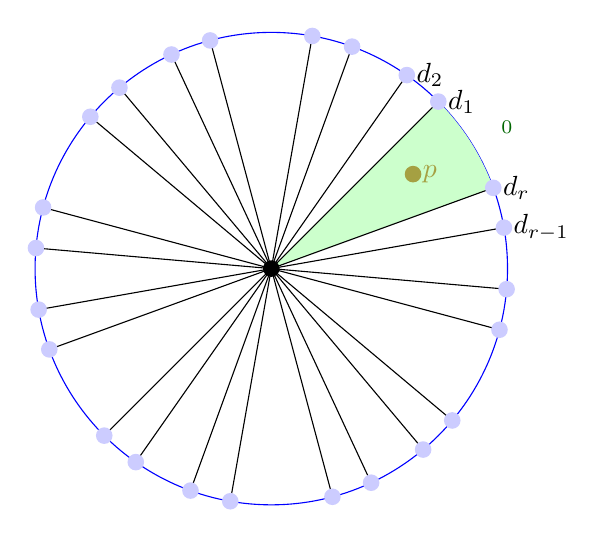
\begin{tikzpicture}[scale=3]
    \node[] (zero) at (0,0) {};
    \draw[blue] (zero) circle (1cm);

    \fill[fill=green!20!white] (0,0) -- ({cos( 20 )},{sin( 20 )}) arc
    (20:45:1) -- cycle;
    \node[green!40!black] at (1.0,0.6) {$\Sect_0$};

    \foreach \w/\str in {10/$d_{r-1}$,
                         20/$d_r$,
                         45/$d_1$,
                         55/$d_2$}
    {\draw (0,0) -- +({cos( \w )},{sin( \w )}) node[right] {\str};
     \fill[blue!20!white] ({cos( \w )},{sin( \w )}) circle (1pt);
     \foreach \sep in {60,120,180,240,300}
     {\draw (0,0) -- +({cos( \w + \sep )},{sin( \w + \sep )});
      \fill[blue!20!white]
        ({cos( \w + \sep )},{sin( \w + \sep )}) circle (1pt);
     }
    };

    \fill[yellow!60!black] (0.6,0.4) circle (1pt);
    \node[yellow!60!black,right] at (0.6,0.4) {$p$};

    \fill (zero) circle (1pt);
  \end{tikzpicture}
\end{center}
Label the first anti-Stokes ray when turning in a positive sense from $p$ as
$d_1$ and label the subsequent rays $d_2,\dots,d_r$ in turn.
\begin{itemize}
  \item Write $\Sect_i:= \Sect(d_i,d_{i+1})$ the ‘ith sector’.
  \begin{itemize}
    \item Note $p \in\Sect_r= \Sect_0$
  \end{itemize}
  \item $\widehat{\Sect}_i:=
    \Sect(d_i-\frac{\pi}{2k-2},d_{1+1}+\frac{\pi}{2k-2})$ the ‘ith supersector’
    \begin{itemize}
      \item The rays bounding these supersectors are usually refered as
        \textcolor{red!40!black}{‘Stokes rays’}.
    \end{itemize}
\end{itemize}
\begin{center}
  \begin{tikzpicture}[scale=3]
    \node[] (zero) at (0,0) {};
    \draw[blue] (zero) circle (1cm);

    \fill[fill=green!20!white] (0,0) -- ({cos( 15 )},{sin( 15 )}) arc
      (15:85:1) -- cycle;

    \fill[fill=red!60!black] (0,0) -- ({cos( 15 )*0.5},{sin( 15 )*0.5}) arc
      (15:45:0.5) -- cycle;
    \fill[fill=red!60!black] (0,0) -- ({cos( 55 )*0.5},{sin( 55 )*0.5}) arc
      (55:85:0.5) -- cycle;

    \fill[fill=green!20!white] (0,0) -- ({cos( 15 )*0.4},{sin( 15 )*0.4}) arc
      (15:85:0.4) -- cycle;

    \node[green!40!black] at (.9,.9) {$\widehat\Sect_1$};

    \node[] (lft) at ({cos( 85 )},{sin( 85 )}) {};
    \node[] (rgt) at ({cos( 15 )},{sin( 15 )}) {};

    \draw[->,red!40!black] ({cos( 45 )},{sin( 45 )})
      to [out=35, in=25] (rgt);

    \draw[->,red!40!black] ({cos( 55 )},{sin( 55 )})
      to [out=65, in=75] (lft);

    \draw[thick,red!40!black,path fading=west] (0,0) -- +({cos( 85 )},{sin( 85 )});
    \draw[thick,red!40!black,path fading=west] (0,0) -- +({cos( 15 )},{sin( 15 )});
    \fill[red!40!black] ({cos( 85 )},{sin( 85 )}) circle (1pt);
    \fill[red!40!black] ({cos( 15 )},{sin( 15 )}) circle (1pt);

    \foreach \w/\str in {10/$d_{r-1}$,
                         20/$d_r$,
                         45/$d_1$,
                         55/$d_2$}
    {\draw (0,0) -- +({cos( \w )},{sin( \w )}) node[right] {\str};
     \fill[blue!20!white] ({cos( \w )},{sin( \w )}) circle (.7pt);
     \foreach \sep in {60,120,180,240,300}
     {\draw (0,0) -- +({cos( \w + \sep )},{sin( \w + \sep )});
      \fill[blue!20!white]
        ({cos( \w + \sep )},{sin( \w + \sep )}) circle (.7pt);
     }
    };

    \fill[yellow!60!black] (0.6,0.4) circle (1pt);
    \node[yellow!60!black,right] at (0.6,0.4) {$p$};

    \fill (zero) circle (1pt);
  \end{tikzpicture}
\end{center}

\subsection{More}
\begin{defn}
  \begin{itemize}
    \item $\Syst(A^0):=\{d-A \mid A=\hat{F}[A^0] \text{ for some } \hat{F}\in
      G\llbracket z\rrbracket\}$\footnote{the set of germs at $0\in\C$ of
      meromorphic connections on the trivial rank $n$ vector bundle, that are
      formally equivalent to $d-A^0$.}
      where
      \begin{itemize}
        \item $A$ is a matrix of germs of meromorphic one-forms
        \item $\hat{F}[A^0]=(d\hat{F})\hat{F}^{-1}+\hat{F}A^0\hat{F}^{-1}$
        \item $G\llbracket z\rrbracket:=\GL_n(\C\llbracket z\rrbracket)$
          \begin{itemize}
            \item does not act on $\Syst(A^0)$
          \end{itemize}
      \end{itemize}
  \end{itemize}
  The group $G\{z\}:=\GL_n(\C\{z\})$ acts on $\Syst(A^0)$,  study
  \begin{center}
    $\Syst(A^0)/G\{z\}$\footnote{The set of isomorphism classes of germs of
    meromorphic connections formally equivalent to $A^0$. Note that any
    generic connection is formally equivalent to some such $A^0$.}
  \end{center}
  In the abelian and the simple pole case this is only a point.
\end{defn}
\begin{defn}
  \begin{itemize}
    \item $\widehat\Syst_{cf}(A^0)$ :\Leftrightarrow the set of compatibly
      framed connection germs with both irregular and formal type $A^0$.
    \item $\widehat\Syst_{mp}(A^0):=\{(A,\hat{F})\mid A\in\Syst(A^0)
      ,\hat{F}\in G\llbracket z\rrbracket
      ,A=\hat{F}[A^0]\}$
      the set of \emph{marked pairs}.
  \end{itemize}
  There is a canonical isomorphism
  $\widehat\Syst_{cf}(A^0)\cong\widehat\Syst_{mp}(A^0)$\footnote{Let
  $\Syst(A^0)$ denote either of these two sets.}.

  $G\{z\}$ action on marked pairs: $g(A,\hat{F})=(g[A],g\circ\hat{F})$
  \[
    \mathcal{H}(A^0):=\widehat\Syst(A^0)/G\{z\}
  \]
\end{defn}
Moreover the actions of $T$ and $G\{z\}$ on $\Syst(A^0)$ commute so
\[
  \Syst(A^0)/G\{z\}\cong\mathcal{H}(A^0)/T \,.
\]

\subsection{Theoremes}
\begin{thm}[1.22 in \cite{thboalch}]
  There is a natural isomorphism
  \[
    \cH(A^0)\cong\prod_{d\in\A}\Sto_d(A^0)
  \]
  and for each choice of $\log(z)$ in the direction $d$ the Stokes group
  $\Sto_d(A^0)$ has a faithfull representation $\rho$ on $\C^n$ inducing an
  isomorphism
  \[
    \rho:\Sto_d(A^0)\to\SSto_d(A^0).
  \]
  In particular each $\Sto_d(A^0)$ and therefore $\cH(A^0)$ is a\dots
\end{thm}
\begin{thm}[3.1, or Prop 1.24 in \cite{thboalch}]
  Let $\hat{F}\in G\llbracket z\rrbracket$ such that $A:=F[A_0]$ has
  convergent entries.
  Set the radius of the sectors $\Sect_i$, $\widehat\Sect_i$ to be less than
  the radius of convergence of $A$.
  Then:
  \begin{enumerate}
    \item On each sector $\Sect_i$ there is a canonical way to choose an
      invertible $n\times n$ matrix of holomorphic Functions
      $\Sigma_i(\hat F)$ such that $\Sigma_i(\hat F)[A^0]=A$
    \item $\Sigma_i(\hat F)$ can be analytically continued to the supersector
      $\widehat\Sect_i$ and then $\Sigma_i(\hat F)$ is asymptotic to $\hat F$
      at $0$ within $\widehat\Sect_i$
    \item If $g\in G\{z\}$ and $t\in T$ then
      $\Sigma_i(g\circ\hat F \circ t^{-1})=g\circ\Sigma_i(\hat F)\circ t^{-1}$.
  \end{enumerate}
\end{thm}
\begin{itemize}
  \item The point is that on a narrow sector there are generally many
    holomorphic isomorphisms between $A_0$ and $A$ which are asymptotic to
    $\hat F$ and one is being chosen in a canonical way
  \item $\Sigma_i(\hat F)$ is in fact uniquely characterised by property 2.
\end{itemize}
\begin{prop}[Prop 1.24 in \cite{thboalch}]
  \begin{enumerate}
  \setcounter{enumi}{2}
  \item If $\hat H\in\hat G$ is the taylor series at $0$ of an analytic gauge
    transformation $H\in G\{z\}$ then
    \[
      \Sigma_i(\hat H \hat F)=H\Sigma_i(\hat F)
      \qquad
      \Sigma_i(\hat F \hat H)=\Sigma_i(\hat F)H
    \]
  \end{enumerate}
\end{prop}
\begin{rem}[1.41 from \cite{thboalch} on pages 16f]
  Note that in most of the recent references we have used, Stokes matrices
  are used to classify
  \begin{itemize}
    \item meromorphic connections within fixed formal \textbf{meromorphic
      classes, modulo meromorphic equivalence}.
  \end{itemize}
  Whereas here we classify
  \begin{itemize}
    \item meromorphic connections within fixed \textbf{formal analytic
      classes, modulo analytic equivalence},
  \end{itemize}
  as is done in the older literature.  The fact is that the sets equivalence
  classes are the same in both cases. It is important for us to work with
  analytic, rather than meromorphic gauge transformations, because then the
  $\C^\infty$ viewpoint in Chapter 3 is cleaner. This distinction relates to
  the difference between \textbf{‘regular singular’} connections and
  \textbf{‘logarithmic’} connections.
\end{rem}
%}}}

\section{Sheaf view: \cite{sabbah2007isomonodromic}} %{{{
\begin{defn}
  Let $(\cM,\nabla)$ be a meromorphic bundle with connection.
  \begin{itemize}
    \item A germ of a $(\cM,\nabla)$ is
      \emph{elementary} if it is isomorphic to some germ
      \[
        (\cE^\phi,\nabla)\otimes(\cR,\nabla)
      \]
      where
      \begin{itemize}
        \item $(\cR,\nabla)$ ha regular singularity along $\{0\}\times X$
      \end{itemize}
    \item $(\cM,\nabla)$ is a \emph{model} if it is isomorphic to a direct sum
      of elementary models, written as
      \[
        \bigoplus_\phi(\cE^\phi\otimes\cR_\phi)
      \]
      where we assume that
      \begin{itemize}
        \item the meromorphic bundles with connection $\cR_\phi$ have regular
          singularity and
        \item the
          $\phi\in\C\{t\textcolor{gray}{\underset{\text{parameter}}
            {\underbrace{,x_1,\ldots,x_n}}}\}[t−1]$
          \begin{itemize}
            \item have no holomorphic part and
            \item are pairwise distinct.
          \end{itemize}
      \end{itemize}
    \item We will say that a model is \emph{good} if,
      \begin{itemize}
        \item for all $\phi\neq\psi$
          \begin{itemize}
            \item such that $\cR_\phi$, $\cR_\psi$ are nonzero,
          \end{itemize}
          the order of the pole along $t=0$ of $(\phi−\psi)(t,x)$ does not
          depend on $x$ being in some neighbourhood of $x^o$.
      \end{itemize}
  \end{itemize}
\end{defn}
\begin{thm}[Formal decomposition (II.5.7)]
  Let $(\cM,\nabla)$ be a germ of meromorphic bundle with connection,
  \begin{itemize}
    \item equipped with a basis 
      \begin{itemize}
        \item 
          in which the matrix $\Omega$ takes the form
          \[
            \Omega=t^{-r}\left[A(t,x)\frac{dt}{t}
              +\sum_{i=1}^nC^{(i)}(t,x)dx_i\right]
          \]
        with
        \begin{itemize}
          \item $r\geq1$
          \item $A$ and the $C^{(i)}$ having holomorphic entries, and
          \item $A_0:=A(0,x^0)$ being regular semisimple\footnote{i.e.\ with
            pairwise distinct eigenvalues.}
        \end{itemize}
      \end{itemize}
  \end{itemize}
  Then there exist
  \begin{itemize}
    \item a good model $(\cM^{good},\nabla)
      =\left(\bigoplus_\phi(\cE^\phi\otimes\cR_\phi) \right)$ and
    \item a \textcolor{red!40!black}{`formal'} isomorphism
      \[
        \textcolor{red!40!black}{\hat\cO_{D\times X,x_0}\otimes}(\cM,\nabla)
        \overset{\sim}{\longrightarrow}
      \textcolor{red!40!black}{\hat\cO_{D\times X,x_0}\otimes}
        \left(\bigoplus_\phi(\cE^\phi\otimes\cR_\phi) \right)
      \]
  \end{itemize}
\end{thm}

%}}}

\section{Local Moduli}
\subsection{\dots / Models}

\begin{paracol}{2} %%%%%%%%%%%%%%%%%%%%%%%%%%%%%%%%%%%%%%%%%%%%%%%%%%%%%%%%%%%%
  \begin{thm}[1.22 in \cite{thboalch}]
    There is a natural isomorphism
    \[
      \cH(A^0)\cong\prod_{d\in\A}\Sto_d(A^0)
    \]
    and for each choice of $\log(z)$ in the direction $d$ the Stokes group
    $\Sto_d(A^0)$ has a faithfull representation $\rho$ on $\C^n$ inducing an
    isomorphism
    \[
      \rho:\Sto_d(A^0)\to\SSto_d(A^0).
    \]
    In particular each $\Sto_d(A^0)$ and therefore $\cH(A^0)$ is a\dots
  \end{thm}

  \switchcolumn{} %%%%%%%%%%%%%%%%%%%%%%%%%%%%%%%%%%%%%%%%%%%%%%%%%%%%%%%%%%%%%
\end{paracol} %%%%%%%%%%%%%%%%%%%%%%%%%%%%%%%%%%%%%%%%%%%%%%%%%%%%%%%%%%%%%%%%%

\subsection{Asymptotic expansions / The sheaf $\cA$}

\subsection{\dots / Sectorial classificaton} %{{{
\begin{paracol}{2} %%%%%%%%%%%%%%%%%%%%%%%%%%%%%%%%%%%%%%%%%%%%%%%%%%%%%%%%%%%%
  \switchcolumn{} %%%%%%%%%%%%%%%%%%%%%%%%%%%%%%%%%%%%%%%%%%%%%%%%%%%%%%%%%%%%%
  Let $\sM$ be a germ at $(0,x^o)$ of a meromorphic bundle with poles along
  $\{0\}\times X$.
  \begin{thm}[II.5.12]
    Let us assume that there exists
    \begin{itemize}
      \item a good model $\sM^{good}$ and
      \item an isomorphism $\hat\lambda: \hat\sM
        \overset{\sim}{\longrightarrow}\hat\sM^{good}$.
    \end{itemize}
    Then,
    \begin{itemize}
      \item for any $e^{i\theta^o}\in S^1$,
    \end{itemize}
    there exists an isomorphism
    \[
      \tilde\lambda_{\theta^o}: \tilde\sM_{\theta^o}
      \overset{\sim}{\longrightarrow}\tilde\sM^{good}_{\theta^o},
    \]
    lifting $\hat\lambda$.
  \end{thm}
  That is, such that the diagram
  \[ \begin{tikzcd}
      \tilde\sM_{\theta^o} \dar \rar{\tilde\lambda_{\theta^o}} &
        \tilde\sM^{good}_{\theta^o} \dar
        \\\hat\sM \rar{\hat\lambda} &
        \hat\sM^{good}
  \end{tikzcd} \]
  commutes.
\end{paracol} %%%%%%%%%%%%%%%%%%%%%%%%%%%%%%%%%%%%%%%%%%%%%%%%%%%%%%%%%%%%%%%%%
%}}}

\subsection{\dots / Stokes sheaf}

\section{Global Moduli}
